\chapter{Vector Algebra}

\section{Vectors and scalars}

\section{Dot product}

\begin{exercise}{1.1}
	Classify the following quantities according to whether they are vectors or scalars: density, magnetic field strength, power, momentum, angular momentum, acceleration.
\end{exercise}

\begin{proof}
	Density, magnetic field strength, power are scalars. Momentum, angular momentum, acceleration are vectors.
\end{proof}

\begin{exercise}{1.2}
	\( \mathbf{a} = (2,0,3) \) and \( \mathbf{b} = (1,0,-1) \), find \( \abs{\mathbf{a}} \), \( \abs{\mathbf{b}} \), \( \mathbf{a} + \mathbf{b} \), \( \mathbf{a} - \mathbf{b} \) and \( \mathbf{a} \cdot \mathbf{b} \). What is the angle between the vectors \( \mathbf{a} \) and \( \mathbf{b} \)?
\end{exercise}

\begin{proof}
	\( \abs{\mathbf{a}} = \sqrt{13} \); \( \abs{\mathbf{b}} = \sqrt{2} \); \( \mathbf{a} + \mathbf{b} = (3, 0, 2) \); \( \mathbf{a} - \mathbf{b} = (1, 0, 4) \); \( \mathbf{a} \cdot \mathbf{b} = -1 \). The angle between the vectors \( \mathbf{a} \) and \( \mathbf{b} \) is \( \arccos\left(-\frac{1}{\sqrt{26}}\right) \).
\end{proof}

\begin{exercise}{1.3}
	If \( \mathbf{u} = (1,2,2) \) and \( \mathbf{v} = (-6,2,3) \), find the component of \( \mathbf{u} \) in the direction of \( \mathbf{v} \) and the component of \( \mathbf{v} \) in the direction of \( \mathbf{u} \).
\end{exercise}

\begin{proof}
	The component of \( \mathbf{u} \) in the direction of \( \mathbf{v} \) is
	\[
		\dfrac{\mathbf{v}\cdot \mathbf{u}}{\abs{\mathbf{v}}^{2}}\mathbf{v} = \dfrac{4}{49} (-6, 2, 3) = \left(-\dfrac{24}{49}, \dfrac{8}{49}, \dfrac{12}{49}\right).
	\]

	The component of \( \mathbf{v} \) in the direction of \( \mathbf{u} \) is
	\[
		\dfrac{\mathbf{u}\cdot \mathbf{v}}{\abs{\mathbf{u}}^{2}}\mathbf{u} = \dfrac{4}{9} (1, 2, 2) = \left(\dfrac{4}{9}, \dfrac{8}{9}, \dfrac{8}{9}\right).
	\]
\end{proof}

\begin{exercise}{1.4}
	Find the equation of the plane that is perpendicular to the vector \( (1,1,-1) \) and passes through the point \( x = 1 \), \( y = 2 \), \( z = 1 \).
\end{exercise}

\begin{proof}
	The equation of the plane is
	\[
		1\cdot x + 1\cdot y + (-1)\cdot z = 1\cdot 1 + 1\cdot 2 + (-1)\cdot 1
	\]

	which is equivalent to
	\[
		x + y - z = 2.
	\]
\end{proof}

\begin{exercise}{1.5}
	Use vector methods to show that the diagonals of a rhombus are perpendicular.
\end{exercise}

\begin{proof}
	Let \( ABCD \) be a rhombus.
	\begingroup
	\allowdisplaybreaks%
	\begin{align*}
		\mathbf{AC} \cdot \mathbf{BD} & = (\mathbf{AB} + \mathbf{AD}) \cdot (\mathbf{AD} - \mathbf{AB})                                    \\
		                              & = \mathbf{AB} \cdot \mathbf{AD} + \mathbf{AD}^{2} - \mathbf{AB}^{2} - \mathbf{AD}\cdot \mathbf{AB} \\
		                              & = AD^{2} - AB^{2} = 0.
	\end{align*}
	\endgroup

	Hence \( AC \) and \( BD \) are perpendicular.
\end{proof}

\begin{exercise}{1.6}
	What is the angle between any two diagonals of a cube?
\end{exercise}

\begin{proof}
	Any two diagonals of a cube are perpendicular.
\end{proof}

\begin{exercise}{1.7}
	Use vectors to show that for any triangle, the three lines drawn from each vertex to the midpoint of the opposite side all pass through the same point.
\end{exercise}

\begin{proof}
	Let \( ABC \) be a triangle, \( D, E, F \) the midpoints of line segments \( BC, CA, AB \) and \( G = \dfrac{1}{3}(A + B + C) \), then
	\begingroup
	\allowdisplaybreaks%
	\begin{align*}
		\mathbf{AG} & = \dfrac{1}{3}(\mathbf{AB} + \mathbf{AC}) = \dfrac{2}{3}\mathbf{AD}, \\
		\mathbf{BG} & = \dfrac{1}{3}(\mathbf{BC} + \mathbf{BA}) = \dfrac{2}{3}\mathbf{BE}, \\
		\mathbf{CG} & = \dfrac{1}{3}(\mathbf{CA} + \mathbf{CB}) = \dfrac{2}{3}\mathbf{CF}.
	\end{align*}
	\endgroup

	Thus \( AD, BE, CF \) pass through \( G \).
\end{proof}

\section{Cross product}

\section{Scalar triple product}

\section{Vector triple product}

\section{Scalar fields and vector fields}

\begin{exercise}{1.8}
	Find the equation of the straight line which passes through the points \( (1, 1, 1) \) and \( (2, 3, 5) \), (a) in parametric form; (b) in cross product form.
\end{exercise}

\begin{proof}
	In parametric form, the equation is
	\[
		(x, y, z) = (1, 1, 1) + \lambda (2 - 1, 3 - 1, 5 - 1) = (1, 1, 1) + \lambda (1, 2, 4).
	\]

	In cross product form, the equation is
	\[
		(x, y, z) \times (1, 2, 4) = (1, 1, 1) \times (1, 2, 4) = (-2, 3, -1).
	\]
\end{proof}

\begin{exercise}{1.9}
	Using vector methods, prove the sine rule,
	\[
		\dfrac{\sin A}{a} = \dfrac{\sin B}{b} = \dfrac{\sin C}{c}
	\]

	and the cosine rule,
	\[
		c^{2} = a^{2} + b^{2} - 2ab\cos C
	\]

	for the triangle with angles \( A, B, C \) and sides \( a, b, c \).
\end{exercise}

\begin{proof}
	The area of the given triangle is equal to
	\begingroup
	\allowdisplaybreaks%
	\begin{align*}
		\dfrac{1}{2}\left\vert \mathbf{AB} \times \mathbf{AC} \right\vert = \dfrac{1}{2} bc \sin A, \\
		\dfrac{1}{2}\left\vert \mathbf{BC} \times \mathbf{BA} \right\vert = \dfrac{1}{2} ca \sin B, \\
		\dfrac{1}{2}\left\vert \mathbf{CA} \times \mathbf{CB} \right\vert = \dfrac{1}{2} ab \sin C.
	\end{align*}
	\endgroup

	Hence \( \dfrac{\sin A}{a} = \dfrac{\sin B}{b} = \dfrac{\sin C}{c} \).

	On the other hand
	\[
		c^{2} = \mathbf{AB}^{2} = {\left(\mathbf{CB} - \mathbf{CA}\right)}^{2} = \mathbf{CB}^{2} + \mathbf{CA}^{2} - 2\mathbf{CB}\cdot \mathbf{CA} = a^{2} + b^{2} - 2ab\cos C.
	\]
\end{proof}

\begin{exercise}{1.10}
	\begin{enumerate}[label={(\alph*)}]
		\item Show that the set of vectors and the operation of vector addition form a group. (The set of objects \( a,b,c,\ldots \) and the operation \( \star \) form a group if the following four conditions are satisfied: (i) for any two elements \( a \) and \( b \), \( a\star b \) is in the set; (ii) \( (a\star b)\star c = a\star(b\star c) \); (iii) there is an element \( I \) obeying \( a\star I=I\star a=a \); (iv) each element \( a \) has an inverse \( a^{-1} \) such that \( a\star a^{-1}=a^{-1}\star a=I \).)
		\item Do the set of vectors and the dot product form a group?
		\item Do the set of vectors and the cross product form a group?
	\end{enumerate}
\end{exercise}

\begin{proof}
	\begin{enumerate}[label={(\alph*)}]
		\item The sum of two vectors is a vector. Vector addition is associative. The zero vector \( \mathbf{0} \) acts as the identity element. For each vector \( \mathbf{a} \), one has \( \mathbf{a} + (-\mathbf{a}) = (-\mathbf{a}) + \mathbf{a} = \mathbf{0} \).
		\item No. The dot product of two vectors is not a vector.
		\item No. The cross product is not associative.
	\end{enumerate}
\end{proof}

\begin{exercise}{1.11}
	Simplify the following expressions:
	\begin{enumerate}[label={(\alph*)}]
		\item \( {\left\vert \mathbf{a} \times \mathbf{b} \right\vert}^{2} + {\left( \mathbf{a} \cdot \mathbf{b} \right)}^{2} \);
		\item \( \mathbf{a} \times (\mathbf{b} \times (\mathbf{a} \times \mathbf{b})) \);
		\item \( (\mathbf{a} - \mathbf{b}) \cdot (\mathbf{b} - \mathbf{c}) \times (\mathbf{c} - \mathbf{a}) \);
		\item \( (\mathbf{a} \times \mathbf{b}) \cdot (\mathbf{b} \times \mathbf{c}) \times (\mathbf{c} \times \mathbf{a}) \).
	\end{enumerate}
\end{exercise}

\begin{proof}
	\begin{enumerate}[label={(\alph*)}]
		\item \begingroup
		      \allowdisplaybreaks%
		      \begin{align*}
			      {\left\vert \mathbf{a} \times \mathbf{b} \right\vert}^{2} + {\left( \mathbf{a} \cdot \mathbf{b} \right)}^{2} = {\left\vert \mathbf{a} \right\vert}^{2} {\left\vert \mathbf{b} \right\vert}^{2} {\left(\sin\left(\mathbf{a}, \mathbf{b}\right)\right)}^{2} + {\left\vert \mathbf{a} \right\vert}^{2} {\left\vert \mathbf{b} \right\vert}^{2} {\left(\cos\left(\mathbf{a}, \mathbf{b}\right)\right)}^{2} = {\left\vert \mathbf{a} \right\vert}^{2} {\left\vert \mathbf{b} \right\vert}^{2}.
		      \end{align*}
		      \endgroup
		\item \begingroup
		      \allowdisplaybreaks%
		      \begin{align*}
			      \mathbf{a} \times (\mathbf{b} \times (\mathbf{a} \times \mathbf{b})) & = (\mathbf{a} \cdot (\mathbf{a} \times \mathbf{b})) \mathbf{b} - (\mathbf{a} \cdot \mathbf{b}) (\mathbf{a} \times \mathbf{b}) \\
			                                                                           & = -(\mathbf{a} \cdot \mathbf{b}) (\mathbf{a} \times \mathbf{b})                                                               \\
			                                                                           & = (\mathbf{a} \cdot \mathbf{b}) (\mathbf{b} \times \mathbf{a}).
		      \end{align*}
		      \endgroup
		\item \( (\mathbf{b} - \mathbf{c}) \times (\mathbf{c} - \mathbf{a}) \) is perpendicular to \( \mathbf{b} - \mathbf{c} \) and \( \mathbf{c} - \mathbf{a} \). So \( (\mathbf{b} - \mathbf{c}) \times (\mathbf{c} - \mathbf{a}) \) is perpendicular to \( \mathbf{a} - \mathbf{b} = -(\mathbf{b} - \mathbf{c}) - (\mathbf{c} - \mathbf{a}) \). Therefore \( (\mathbf{a} - \mathbf{b}) \cdot (\mathbf{b} - \mathbf{c}) \times (\mathbf{c} - \mathbf{a}) = 0 \).
		\item \begingroup
		      \allowdisplaybreaks%
		      \begin{align*}
			      (\mathbf{a} \times \mathbf{b}) \cdot (\mathbf{b} \times \mathbf{c}) \times (\mathbf{c} \times \mathbf{a}) & = (\mathbf{a} \times \mathbf{b}) \cdot \left( ((\mathbf{b} \times \mathbf{c})\cdot \mathbf{a})\mathbf{c} - ((\mathbf{b} \times \mathbf{c}) \cdot \mathbf{c})\mathbf{a} \right) \\
			                                                                                                                & = (\mathbf{a} \times \mathbf{b}) \cdot (((\mathbf{b} \times \mathbf{c}) \cdot \mathbf{a})\mathbf{c})                                                                           \\
			                                                                                                                & = ((\mathbf{b} \times \mathbf{c})\cdot \mathbf{a})((\mathbf{a} \times \mathbf{b})\cdot \mathbf{c})                                                                             \\
			                                                                                                                & = {(\mathbf{a}\cdot(\mathbf{b} \times \mathbf{c}))}^{2}.
		      \end{align*}
		      \endgroup

		      The last line is true due to \( (\mathbf{b} \times \mathbf{c})\cdot \mathbf{a} = (\mathbf{a} \times \mathbf{b}) \cdot \mathbf{c} \).
	\end{enumerate}
\end{proof}

\begin{exercise}{1.12}
	The vector \( \mathbf{x} \) obeys the two equations \( \mathbf{x} \cdot \mathbf{a} = 1 \) and \( \mathbf{x} \times \mathbf{a} = \mathbf{b} \), where \( \mathbf{a} \) and \( \mathbf{b} \) are constant vectors. Solve these equations to find an expression for \( \mathbf{x} \) in terms of \( \mathbf{a} \) and \( \mathbf{b} \). Give a geometrical interpretation of this question.
\end{exercise}

\begin{proof}
	\( \mathbf{a} \times \mathbf{b} = \mathbf{a} \times (\mathbf{x} \times \mathbf{a}) = (\mathbf{a}\cdot \mathbf{a})\mathbf{x} - (\mathbf{a}\cdot\mathbf{x})\mathbf{a} = {\left\vert \mathbf{a} \right\vert}^{2}\mathbf{x} - \mathbf{a} \). Therefore
	\[
		\mathbf{x} = \dfrac{1}{{\left\vert\mathbf{a}\right\vert}^{2}} \mathbf{a} \times \mathbf{b} - \dfrac{1}{{\left\vert\mathbf{a}\right\vert}^{2}}\mathbf{a}.
	\]

	\( \mathbf{x} \) is the vector that is perpendicular to \( \mathbf{b} \) such that \( \mathbf{x}, \mathbf{a}, \mathbf{b} \) follow the right-hand rule and \( \left\vert \mathbf{x}\right\vert \cos(\mathbf{x}, \mathbf{a}) = \dfrac{1}{\left\vert \mathbf{a} \right\vert} \); \( \left\vert \mathbf{x}\right\vert \sin(\mathbf{x}, \mathbf{a}) = \dfrac{\left\vert \mathbf{b} \right\vert}{\left\vert \mathbf{a} \right\vert} \).
\end{proof}

\begin{exercise}{1.13}
	Find the equation of the line on which the two planes \( \mathbf{r} \cdot \mathbf{a} = 1 \) and \( \mathbf{r} \cdot \mathbf{b} = 1 \) meet.
\end{exercise}

\begin{proof}
	\[
		\mathbf{r} \times (\mathbf{a} \times \mathbf{b}) = (\mathbf{r}\cdot \mathbf{b}) \mathbf{a} - (\mathbf{r}\cdot \mathbf{a}) \mathbf{b} = \mathbf{a} - \mathbf{b}.
	\]

	This is the cross product equation for the straight line which is the intersection of two planes \( \mathbf{r} \cdot \mathbf{a} = 1 \) and \( \mathbf{r} \cdot \mathbf{b} = 1 \).
\end{proof}

\begin{exercise}{1.14}
	\begin{enumerate}[itemsep=0pt,label={(\alph*)}]
		\item Express the vector \( \mathbf{a} \times \mathbf{b} \) in the form of \( \alpha\mathbf{a} + \beta\mathbf{b} + \gamma\mathbf{c} \), assuming that the vectors \( \mathbf{a}, \mathbf{b}, \) and \( \mathbf{c} \) are not coplanar.
		\item Hence find an expression for \( {(\mathbf{a} \times \mathbf{b} \cdot \mathbf{c})}^{2} \) that does not involve any cross products.
		\item Hence find the volume of a tetrahedron made from four equilateral triangles with sides of length \( 1 \).
	\end{enumerate}
\end{exercise}

\begin{proof}
	\begin{enumerate}[itemsep=0pt,label={(\alph*)}]
		\item Conduct the Gram-Schmidt process:
		      \[
			      \mathbf{u} = \mathbf{a};  \mathbf{v} = \mathbf{b} - \dfrac{\mathbf{b} \cdot \mathbf{u}}{{\abs{\mathbf{u}}}^{2}} \mathbf{u}; \mathbf{w} = \mathbf{c} - \dfrac{\mathbf{c} \cdot \mathbf{v}}{{\abs{\mathbf{v}}}^{2}}\mathbf{v} - \dfrac{\mathbf{c}\cdot\mathbf{u}}{{\abs{\mathbf{u}}}^{2}}\mathbf{u}.
		      \]

		      Let \( \mathbf{e_{1}} = \dfrac{\mathbf{u}}{\abs{\mathbf{u}}} \); \( \mathbf{e_{2}} = \dfrac{\mathbf{v}}{\abs{\mathbf{v}}} \); \( \mathbf{e_{3}} = \dfrac{\mathbf{w}}{\abs{\mathbf{w}}} \).

		      \( \mathbf{a} \times \mathbf{b} = (\mathbf{a} \times \mathbf{b} \cdot \mathbf{e_{1}})\mathbf{e_{1}} + (\mathbf{a} \times \mathbf{b} \cdot \mathbf{e_{2}})\mathbf{e_{2}} + (\mathbf{a} \times \mathbf{b} \cdot \mathbf{e_{3}})\mathbf{e_{3}} \). However, \( (\mathbf{a} \times \mathbf{b} \cdot \mathbf{e_{1}}) = (\mathbf{a} \times \mathbf{b} \cdot \mathbf{e_{2}}) = 0 \).
		      \begingroup
		      \allowdisplaybreaks%
		      \begin{align*}
			      {\abs{\mathbf{u}}}^{2} & = {\abs{\mathbf{a}}}^{2};                                                                                                                                                                                                                                                                                                                                                                                                                                           \\
			      {\abs{\mathbf{v}}}^{2} & = {\abs{\mathbf{b}}}^{2} + \dfrac{{(\mathbf{b}\cdot \mathbf{u})}^{2}}{\abs{\mathbf{u}}^{2}} - \dfrac{2{(\mathbf{b}\cdot \mathbf{u})}^{2}}{\abs{\mathbf{u}}^{2}} =  {\abs{\mathbf{b}}}^{2} - \dfrac{{(\mathbf{b}\cdot \mathbf{u})}^{2}}{\abs{\mathbf{u}}^{2}};                                                                                                                                                                                                       \\
			      {\abs{\mathbf{w}}}^{2} & = {\abs{\mathbf{c}}}^{2} - \dfrac{{(\mathbf{c}\cdot \mathbf{v})}^{2}}{\abs{\mathbf{v}}^{2}} - \dfrac{{(\mathbf{c}\cdot \mathbf{u})}^{2}}{\abs{\mathbf{u}}^{2}}                                                                                                                                                                                                                                                                                                      \\
			                             & = {\abs{\mathbf{c}}}^{2} - \dfrac{{(\mathbf{c}\cdot \mathbf{b})}^{2} + \dfrac{{(\mathbf{b} \cdot \mathbf{a})}^{2} {(\mathbf{c}\cdot \mathbf{a})}^{2}}{{\abs{\mathbf{a}}}^{4}} - \dfrac{2 (\mathbf{c}\cdot\mathbf{b})(\mathbf{b}\cdot\mathbf{a})(\mathbf{c}\cdot\mathbf{a})}{{\abs{\mathbf{a}}}^{2}}}{ {\abs{\mathbf{b}}}^{2} - \dfrac{{(\mathbf{b}\cdot \mathbf{a})}^{2}}{\abs{\mathbf{a}}^{2}}} - \dfrac{{(\mathbf{c}\cdot \mathbf{a})}^{2}}{\abs{\mathbf{a}}^{2}} \\
			                             & = {\abs{\mathbf{c}}}^{2} - \dfrac{\abs{\mathbf{a}}^{2} {(\mathbf{c}\cdot\mathbf{b})}^{2} + \dfrac{{(\mathbf{b} \cdot \mathbf{a})}^{2} {(\mathbf{c}\cdot \mathbf{a})}^{2}}{{\abs{\mathbf{a}}}^{2}} - {2 (\mathbf{c}\cdot\mathbf{b})(\mathbf{b}\cdot\mathbf{a})(\mathbf{c}\cdot\mathbf{a})}}{{\abs{\mathbf{b}}}^{2}{\abs{\mathbf{a}}}^{2} - {(\mathbf{b}\cdot\mathbf{a})}^{2}} - \dfrac{{(\mathbf{c}\cdot \mathbf{a})}^{2}}{\abs{\mathbf{a}}^{2}}                     \\
			                             & = \dfrac{{\abs{\mathbf{a}}}^{2}{\abs{\mathbf{b}}}^{2}{\abs{\mathbf{c}}}^{2} - {\abs{\mathbf{a}}}^{2} {(\mathbf{b}\cdot\mathbf{c})}^{2} - {\abs{\mathbf{b}}}^{2} {(\mathbf{c}\cdot\mathbf{a})}^{2} - {\abs{\mathbf{c}}}^{2} {(\mathbf{a}\cdot\mathbf{b})}^{2} + 2(\mathbf{b}\cdot\mathbf{c})(\mathbf{c}\cdot\mathbf{a})(\mathbf{a}\cdot\mathbf{b})}{{\abs{\mathbf{b}}}^{2}{\abs{\mathbf{a}}}^{2} - {(\mathbf{b}\cdot\mathbf{a})}^{2}}.
		      \end{align*}
		      \endgroup

		      On the other hand
		      \begingroup
		      \allowdisplaybreaks%
		      \begin{align*}
			      \mathbf{w} & = \mathbf{c} - \dfrac{\mathbf{c}\cdot\mathbf{a} + \mathbf{c}\cdot\mathbf{b} - \dfrac{(\mathbf{b}\cdot \mathbf{a})(\mathbf{c}\cdot \mathbf{a})}{{\abs{\mathbf{a}}}^{2}}}{{\abs{\mathbf{b}}}^{2} - \dfrac{{(\mathbf{b}\cdot \mathbf{a})}^{2}}{{\abs{\mathbf{a}}}^{2}}} \left(\mathbf{b} - \dfrac{\mathbf{b}\cdot\mathbf{a}}{{\abs{\mathbf{a}}}^{2}} \mathbf{a}\right) - \dfrac{\mathbf{c}\cdot\mathbf{a}}{{\abs{\mathbf{a}}}^{2}}\mathbf{a}     \\
			                 & = \mathbf{c} - \dfrac{{\abs{\mathbf{a}}}^{2}(\mathbf{c}\cdot\mathbf{a}) + {\abs{\mathbf{a}}}^{2}(\mathbf{c}\cdot\mathbf{b}) - (\mathbf{b}\cdot\mathbf{a})(\mathbf{c}\cdot\mathbf{a}) }{{\abs{\mathbf{b}}}^{2}{\abs{\mathbf{a}}}^{2} - {(\mathbf{b}\cdot\mathbf{a})}^{2}}\left(\mathbf{b} - \dfrac{\mathbf{b}\cdot\mathbf{a}}{{\abs{\mathbf{a}}}^{2}} \mathbf{a}\right) -  \dfrac{\mathbf{c}\cdot\mathbf{a}}{{\abs{\mathbf{a}}}^{2}}\mathbf{a} \\
			                 & = \mathbf{c} + \dfrac{-{\abs{\mathbf{a}}}^{2}(\mathbf{c}\cdot\mathbf{a}) - {\abs{\mathbf{a}}}^{2}(\mathbf{c}\cdot\mathbf{b}) + (\mathbf{b}\cdot\mathbf{a})(\mathbf{c}\cdot\mathbf{a}) }{{\abs{\mathbf{b}}}^{2}{\abs{\mathbf{a}}}^{2} - {(\mathbf{b}\cdot\mathbf{a})}^{2}}\mathbf{b}                                                                                                                                                           \\
			                 & \phantom{=} + \left(  \dfrac{{\abs{\mathbf{a}}}^{2}(\mathbf{c}\cdot\mathbf{a}) + {\abs{\mathbf{a}}}^{2}(\mathbf{c}\cdot\mathbf{b}) - (\mathbf{b}\cdot\mathbf{a})(\mathbf{c}\cdot\mathbf{a}) }{{\abs{\mathbf{b}}}^{2}{\abs{\mathbf{a}}}^{2} - {(\mathbf{b}\cdot\mathbf{a})}^{2}}\dfrac{\mathbf{b}\cdot\mathbf{a}}{{\abs{\mathbf{a}}}^{2}} - \dfrac{\mathbf{c}\cdot\mathbf{a}}{{\abs{\mathbf{a}}}^{2}} \right)\mathbf{a}
		      \end{align*}
		      \endgroup

		      so
		      \begingroup
		      \allowdisplaybreaks%
		      \begin{align*}
			      \mathbf{a} \times \mathbf{b} & = (\mathbf{a} \times \mathbf{b} \cdot \mathbf{e_{3}})\mathbf{e_{3}} = (\mathbf{a} \times \mathbf{b} \cdot \mathbf{w})\dfrac{\mathbf{w}}{{\abs{\mathbf{w}}}^{2}} \\
			                                   & = (\mathbf{a} \times \mathbf{b}\cdot \mathbf{c}) \dfrac{\mathbf{w}}{{\abs{\mathbf{w}}}^{2}}.
		      \end{align*}
		      \endgroup
		\item From part (a), it follows that
		      \begingroup
		      \allowdisplaybreaks%
		      \begin{align*}
			      {(\mathbf{a} \times \mathbf{b} \cdot \mathbf{c})}^{2} = {\abs{\mathbf{a}}}^{2}{\abs{\mathbf{b}}}^{2}{\abs{\mathbf{c}}}^{2} - {\abs{\mathbf{a}}}^{2} {(\mathbf{b}\cdot\mathbf{c})}^{2} - {\abs{\mathbf{b}}}^{2} {(\mathbf{c}\cdot\mathbf{a})}^{2} - {\abs{\mathbf{c}}}^{2} {(\mathbf{a}\cdot\mathbf{b})}^{2} + 2(\mathbf{b}\cdot\mathbf{c})(\mathbf{c}\cdot\mathbf{a})(\mathbf{a}\cdot\mathbf{b}).
		      \end{align*}
		      \endgroup
		\item The volume of a regular tetrahedron of sidelength \( 1 \) is equal to \( \dfrac{1}{6\sqrt{2}} = \dfrac{\sqrt{2}}{12} \).
	\end{enumerate}
\end{proof}

\begin{exercise}{1.15}
	A particle of mass \( m \) at position \( r \) and moving with velocity \( \mathbf{v} \) is subject to a force \( \mathbf{F} \) directed towards the origin, \( \mathbf{F} = -f(\mathbf{r}) \mathbf{r} \). Show that the angular momentum vector \( \mathbf{h} = m\mathbf{r} \times \mathbf{v} \) is constant.
\end{exercise}

\begin{proof}
	Using the coordinate formula of cross product, one can show that \( \dot{\mathbf{h}} = m\dot{\mathbf{r}} \times \mathbf{v} + m\mathbf{r} \times \dot{\mathbf{v}} \).

	According to Newton's law of acceleration
	\[ m\mathbf{r} \times \dot{\mathbf{v}} = m\mathbf{r} \times \mathbf{a} = \mathbf{r} \times \mathbf{F} = \mathbf{r} \times (-f(\mathbf{r})\mathbf{r}) = \mathbf{0}. \]

	Moreover, \( \dot{\mathbf{r}} = \mathbf{v} \) so \( m\dot{\mathbf{r}} \times \mathbf{v} = m\mathbf{v} \times \mathbf{v} = \mathbf{0} \).

	Hence \( \dot{\mathbf{h}} = \mathbf{0} \), which implies that the angular momentum vector \( \mathbf{h} \) is constant.
\end{proof}

\begin{exercise}{1.16}
	Sketch the scalar field \( T(x, y) = x^{2} - y \).
\end{exercise}

\begin{proof}
	The following sketch the scalar field \( T(x, y) = x^{2} - y \).
	\begin{center}
		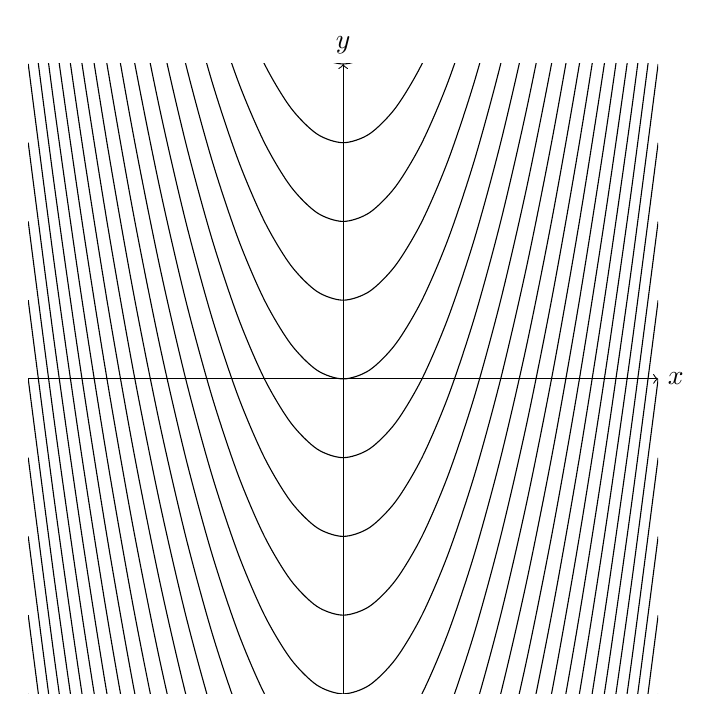
\begin{tikzpicture}
			\draw[->] (-4,0) -- (4,0) node[right] {\(x\)};
			\draw[->] (0,-4) -- (0,4) node[above] {\(y\)};
			\clip (-4,-4) rectangle (4,4);
			\foreach \k in {-20,...,4} {
					\draw[domain=-4:4, smooth, variable=\x] plot ({\x}, {\x*\x + \k});
				}
		\end{tikzpicture}
	\end{center}
\end{proof}

\begin{exercise}{1.17}
	Sketch the vector field \( \mathbf{u}(x, y) = (x + y, -x) \).
\end{exercise}

\begin{proof}
	The following sketch the vector field \( \mathbf{u}(x, y) = (x + y, -x) \).
	\begin{center}
		\begin{tikzpicture}
			\tikzmath{\k = 0.5;}
			\draw[->] (-4,0) -- (4,0) node[right] {\(x\)};
			\draw[->] (0,-4) -- (0,4) node[above] {\(y\)};
			\clip (-4,-4) rectangle (4,4);
			\foreach \x in {-8,-7,...,8} {
					\foreach \y in {-8,-7,...,8} {
							\draw[-Stealth] ({\k*\x},{\k*\y}) -- ({\k*(\x + \x + \y)}, {\k*(\y - \x)});
						}
				}
		\end{tikzpicture}
	\end{center}
\end{proof}
